\documentclass{standalone}
\usepackage{tikz}
\usetikzlibrary{patterns, positioning}


\begin{document}
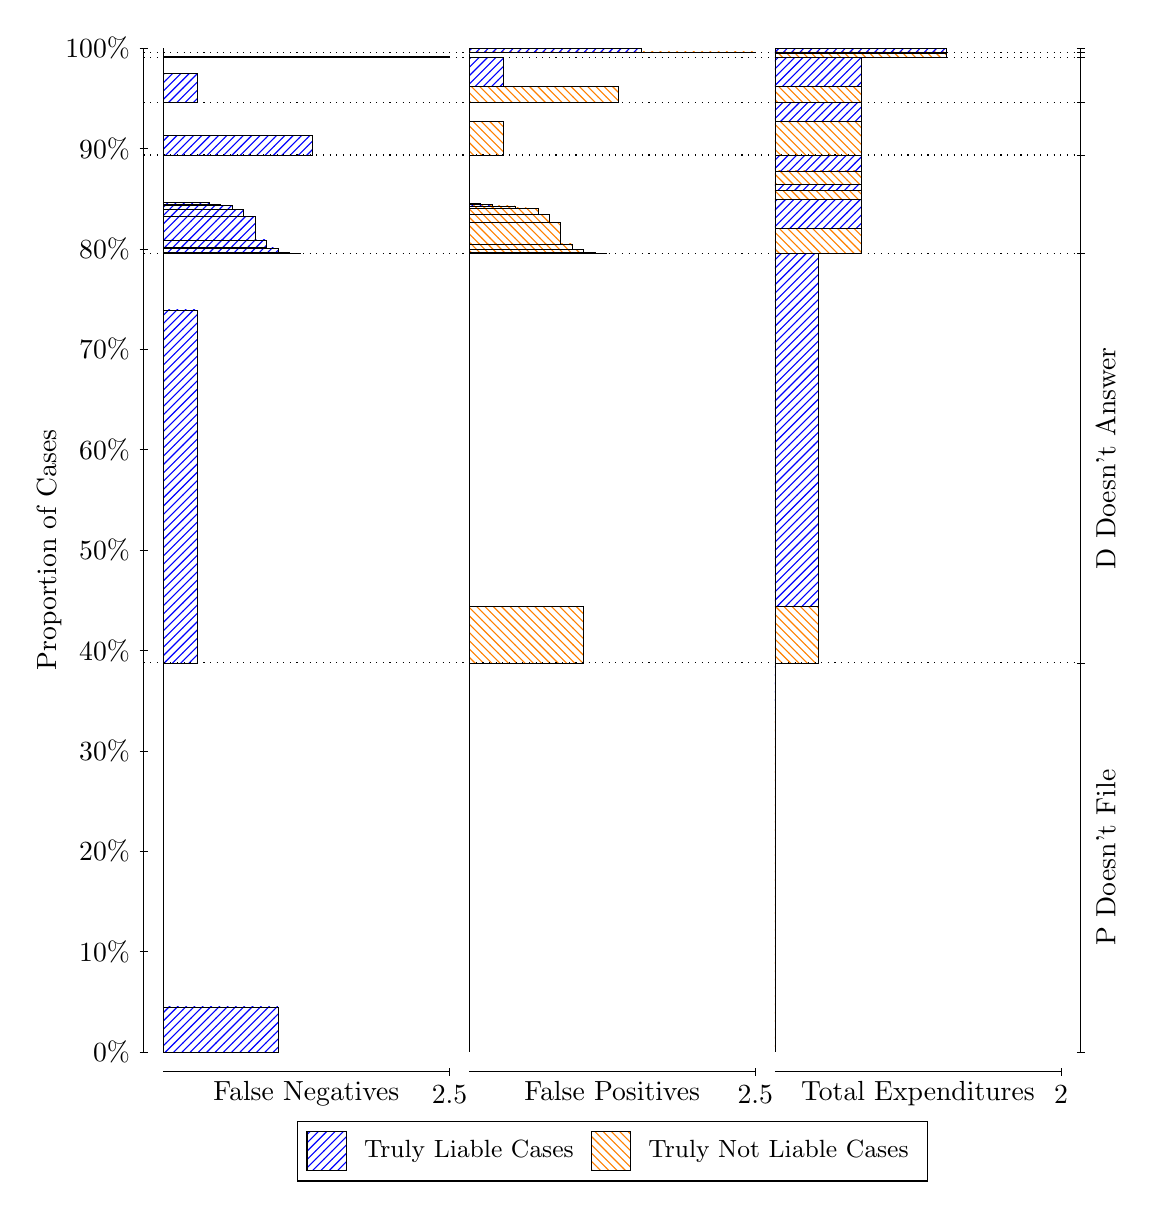
\begin{tikzpicture}
\draw[black, very thin] (1.5,1.75) -- (1.5,14.5);
\node[rotate=90, text=black, anchor=center] at (0.3, 8.125) {Proportion of Cases};
\draw[black, very thin] (1.45,1.75) -- (1.55,1.75);
\node[text=black, anchor=east] at (1.45, 1.75) {0\%};
\draw[black, very thin] (1.45,3.025) -- (1.55,3.025);
\node[text=black, anchor=east] at (1.45, 3.025) {10\%};
\draw[black, very thin] (1.45,4.3) -- (1.55,4.3);
\node[text=black, anchor=east] at (1.45, 4.3) {20\%};
\draw[black, very thin] (1.45,5.575) -- (1.55,5.575);
\node[text=black, anchor=east] at (1.45, 5.575) {30\%};
\draw[black, very thin] (1.45,6.85) -- (1.55,6.85);
\node[text=black, anchor=east] at (1.45, 6.85) {40\%};
\draw[black, very thin] (1.45,8.125) -- (1.55,8.125);
\node[text=black, anchor=east] at (1.45, 8.125) {50\%};
\draw[black, very thin] (1.45,9.4) -- (1.55,9.4);
\node[text=black, anchor=east] at (1.45, 9.4) {60\%};
\draw[black, very thin] (1.45,10.675) -- (1.55,10.675);
\node[text=black, anchor=east] at (1.45, 10.675) {70\%};
\draw[black, very thin] (1.45,11.95) -- (1.55,11.95);
\node[text=black, anchor=east] at (1.45, 11.95) {80\%};
\draw[black, very thin] (1.45,13.225) -- (1.55,13.225);
\node[text=black, anchor=east] at (1.45, 13.225) {90\%};
\draw[black, very thin] (1.45,14.5) -- (1.55,14.5);
\node[text=black, anchor=east] at (1.45, 14.5) {100\%};

\draw[black, very thin] (13.4,1.75) -- (13.4,14.5);
\draw[black, very thin] (13.35,1.75) -- (13.45,1.75);
\node[anchor=west] at (13.35, 1.75) {};
\draw[black, very thin] (13.35,6.6913) -- (13.45,6.6913);
\node[anchor=west] at (13.35, 6.6913) {};
\draw[black, very thin] (13.35,11.889) -- (13.45,11.889);
\node[anchor=west] at (13.35, 11.889) {};
\draw[black, very thin] (13.35,13.141) -- (13.45,13.141);
\node[anchor=west] at (13.35, 13.141) {};
\draw[black, very thin] (13.35,13.812) -- (13.45,13.812);
\node[anchor=west] at (13.35, 13.812) {};
\draw[black, very thin] (13.35,14.378) -- (13.45,14.378);
\node[anchor=west] at (13.35, 14.378) {};
\draw[black, very thin] (13.35,14.44) -- (13.45,14.44);
\node[anchor=west] at (13.35, 14.44) {};
\draw[black, very thin] (13.35,14.5) -- (13.45,14.5);
\node[anchor=west] at (13.35, 14.5) {};

\draw[black, very thin, pattern color=blue, pattern=north east lines] (1.75,1.75) rectangle (3.2033,2.3233);
\draw[black, very thin, pattern color=orange, pattern=north west lines] (1.75,2.3233) rectangle (1.75,6.6913);
\draw[black, very thin, pattern color=blue, pattern=north east lines] (1.75,6.6913) rectangle (2.186,11.173);
\draw[black, very thin, pattern color=orange, pattern=north west lines] (1.75,11.173) rectangle (1.75,11.889);
\draw[black, very thin, pattern color=blue, pattern=north east lines] (1.75,11.889) rectangle (3.494,11.894);
\draw[black, very thin, pattern color=blue, pattern=north east lines] (1.75,11.894) rectangle (3.3487,11.9);
\draw[black, very thin, pattern color=blue, pattern=north east lines] (1.75,11.9) rectangle (3.2033,11.962);
\draw[black, very thin, pattern color=blue, pattern=north east lines] (1.75,11.962) rectangle (3.058,11.965);
\draw[black, very thin, pattern color=blue, pattern=north east lines] (1.75,11.965) rectangle (3.058,12.063);
\draw[black, very thin, pattern color=blue, pattern=north east lines] (1.75,12.063) rectangle (2.9127,12.365);
\draw[black, very thin, pattern color=blue, pattern=north east lines] (1.75,12.365) rectangle (2.7673,12.447);
\draw[black, very thin, pattern color=blue, pattern=north east lines] (1.75,12.447) rectangle (2.622,12.501);
\draw[black, very thin, pattern color=blue, pattern=north east lines] (1.75,12.501) rectangle (2.4767,12.513);
\draw[black, very thin, pattern color=blue, pattern=north east lines] (1.75,12.513) rectangle (2.3313,12.536);
\draw[black, very thin, pattern color=orange, pattern=north west lines] (1.75,12.536) rectangle (1.75,13.141);
\draw[black, very thin, pattern color=blue, pattern=north east lines] (1.75,13.141) rectangle (3.6393,13.389);
\draw[black, very thin, pattern color=orange, pattern=north west lines] (1.75,13.389) rectangle (1.75,13.812);
\draw[black, very thin, pattern color=blue, pattern=north east lines] (1.75,13.812) rectangle (2.186,14.177);
\draw[black, very thin, pattern color=orange, pattern=north west lines] (1.75,14.177) rectangle (1.75,14.378);
\draw[black, very thin, pattern color=blue, pattern=north east lines] (1.75,14.378) rectangle (5.3833,14.389);
\draw[black, very thin, pattern color=orange, pattern=north west lines] (1.75,14.389) rectangle (1.75,14.44);
\draw[black, very thin, pattern color=orange, pattern=north west lines] (1.75,14.44) rectangle (1.75,14.451);
\draw[black, very thin, pattern color=blue, pattern=north east lines] (1.75,14.451) rectangle (1.75,14.5);
\draw[black, very thin, pattern color=orange, pattern=north west lines] (5.6333,1.75) rectangle (5.6333,6.118);
\draw[black, very thin, pattern color=blue, pattern=north east lines] (5.6333,6.118) rectangle (5.6333,6.6913);
\draw[black, very thin, pattern color=orange, pattern=north west lines] (5.6333,6.6913) rectangle (7.0867,7.4076);
\draw[black, very thin, pattern color=blue, pattern=north east lines] (5.6333,7.4076) rectangle (5.6333,11.889);
\draw[black, very thin, pattern color=orange, pattern=north west lines] (5.6333,11.889) rectangle (7.3773,11.894);
\draw[black, very thin, pattern color=orange, pattern=north west lines] (5.6333,11.894) rectangle (7.232,11.901);
\draw[black, very thin, pattern color=orange, pattern=north west lines] (5.6333,11.901) rectangle (7.0867,11.941);
\draw[black, very thin, pattern color=orange, pattern=north west lines] (5.6333,11.941) rectangle (6.9413,12.013);
\draw[black, very thin, pattern color=orange, pattern=north west lines] (5.6333,12.013) rectangle (6.796,12.288);
\draw[black, very thin, pattern color=orange, pattern=north west lines] (5.6333,12.288) rectangle (6.6507,12.386);
\draw[black, very thin, pattern color=orange, pattern=north west lines] (5.6333,12.386) rectangle (6.5053,12.459);
\draw[black, very thin, pattern color=orange, pattern=north west lines] (5.6333,12.459) rectangle (6.36,12.47);
\draw[black, very thin, pattern color=orange, pattern=north west lines] (5.6333,12.47) rectangle (6.2147,12.495);
\draw[black, very thin, pattern color=blue, pattern=north east lines] (5.6333,12.495) rectangle (5.924,12.518);
\draw[black, very thin, pattern color=blue, pattern=north east lines] (5.6333,12.518) rectangle (5.7787,12.53);
\draw[black, very thin, pattern color=blue, pattern=north east lines] (5.6333,12.53) rectangle (5.6333,13.141);
\draw[black, very thin, pattern color=orange, pattern=north west lines] (5.6333,13.141) rectangle (6.0693,13.564);
\draw[black, very thin, pattern color=blue, pattern=north east lines] (5.6333,13.564) rectangle (5.6333,13.812);
\draw[black, very thin, pattern color=orange, pattern=north west lines] (5.6333,13.812) rectangle (7.5227,14.012);
\draw[black, very thin, pattern color=blue, pattern=north east lines] (5.6333,14.012) rectangle (6.0693,14.378);
\draw[black, very thin, pattern color=orange, pattern=north west lines] (5.6333,14.378) rectangle (5.6333,14.429);
\draw[black, very thin, pattern color=blue, pattern=north east lines] (5.6333,14.429) rectangle (5.6333,14.44);
\draw[black, very thin, pattern color=orange, pattern=north west lines] (5.6333,14.44) rectangle (9.2667,14.451);
\draw[black, very thin, pattern color=blue, pattern=north east lines] (5.6333,14.451) rectangle (7.8133,14.5);
\draw[black, very thin, pattern color=orange, pattern=north west lines] (9.5167,1.75) rectangle (9.5167,6.118);
\draw[black, very thin, pattern color=blue, pattern=north east lines] (9.5167,6.118) rectangle (9.5167,6.6913);
\draw[black, very thin, pattern color=orange, pattern=north west lines] (9.5167,6.6913) rectangle (10.062,7.4076);
\draw[black, very thin, pattern color=blue, pattern=north east lines] (9.5167,7.4076) rectangle (10.062,11.889);
\draw[black, very thin, pattern color=orange, pattern=north west lines] (9.5167,11.889) rectangle (10.607,12.212);
\draw[black, very thin, pattern color=blue, pattern=north east lines] (9.5167,12.212) rectangle (10.607,12.581);
\draw[black, very thin, pattern color=orange, pattern=north west lines] (9.5167,12.581) rectangle (10.607,12.693);
\draw[black, very thin, pattern color=blue, pattern=north east lines] (9.5167,12.693) rectangle (10.607,12.769);
\draw[black, very thin, pattern color=orange, pattern=north west lines] (9.5167,12.769) rectangle (10.607,12.939);
\draw[black, very thin, pattern color=blue, pattern=north east lines] (9.5167,12.939) rectangle (10.607,13.141);
\draw[black, very thin, pattern color=orange, pattern=north west lines] (9.5167,13.141) rectangle (10.607,13.564);
\draw[black, very thin, pattern color=blue, pattern=north east lines] (9.5167,13.564) rectangle (10.607,13.812);
\draw[black, very thin, pattern color=orange, pattern=north west lines] (9.5167,13.812) rectangle (10.607,14.012);
\draw[black, very thin, pattern color=blue, pattern=north east lines] (9.5167,14.012) rectangle (10.607,14.378);
\draw[black, very thin, pattern color=orange, pattern=north west lines] (9.5167,14.378) rectangle (11.697,14.429);
\draw[black, very thin, pattern color=blue, pattern=north east lines] (9.5167,14.429) rectangle (11.697,14.44);
\draw[black, very thin, pattern color=orange, pattern=north west lines] (9.5167,14.44) rectangle (11.697,14.451);
\draw[black, very thin, pattern color=blue, pattern=north east lines] (9.5167,14.451) rectangle (11.697,14.5);
\draw[black, dotted] (1.5,6.6913) -- (13.4,6.6913);
\draw[black, dotted] (1.5,11.889) -- (13.4,11.889);
\draw[black, dotted] (1.5,13.141) -- (13.4,13.141);
\draw[black, dotted] (1.5,13.812) -- (13.4,13.812);
\draw[black, dotted] (1.5,14.378) -- (13.4,14.378);
\draw[black, dotted] (1.5,14.44) -- (13.4,14.44);
\draw[black, very thin] (1.75,1.5) -- (5.3833,1.5);
\node[text=black, anchor=north] at (3.5667, 1.5) {False Negatives};
\draw[black, very thin] (5.3833,1.45) -- (5.3833,1.55);
\node[text=black, anchor=north] at (5.3833, 1.45) {2.5};

\draw[black, very thin] (5.6333,1.5) -- (9.2667,1.5);
\node[text=black, anchor=north] at (7.45, 1.5) {False Positives};
\draw[black, very thin] (9.2667,1.45) -- (9.2667,1.55);
\node[text=black, anchor=north] at (9.2667, 1.45) {2.5};

\draw[black, very thin] (9.5167,1.5) -- (13.15,1.5);
\node[text=black, anchor=north] at (11.333, 1.5) {Total Expenditures};
\draw[black, very thin] (13.15,1.45) -- (13.15,1.55);
\node[text=black, anchor=north] at (13.15, 1.45) {2};

\node[text=black, centered, rotate=90] at (13.72, 4.2206) {P Doesn't File};
\node[text=black, centered, rotate=90] at (13.72, 9.2903) {D Doesn't Answer};






\draw (7.449999999999999,1.5) node[draw=none] (baseCoordinate) {};
\begin{scope}[align=center]
        \matrix[scale=0.5, draw=black, below=0.5cm of baseCoordinate, nodes={draw}, column sep=0.1cm]{
            \node[rectangle, draw, minimum width=0.5cm, minimum height=0.5cm, pattern color=blue, pattern=north east lines] {}; &
            \node[draw=none, font=\small, text=black] (B) {Truly Liable Cases}; &
            \node[rectangle, draw, minimum width=0.5cm, minimum height=0.5cm, pattern color=orange, pattern=north west lines] {}; &
            \node[draw=none, font=\small, text=black] (B) {Truly Not Liable Cases}; \\
            };
\end{scope}

\end{tikzpicture}
\end{document}